\documentclass{article}

\usepackage[utf8]{inputenc}
\usepackage[provide=*,french]{babel}
\usepackage[numbers]{natbib}
\usepackage{hyperref}
\usepackage{graphicx}
\usepackage{amsmath,amssymb,amsthm}
\usepackage{enumitem}
\usepackage{geometry}
\geometry{left = 1in, right = 1in, top = 1in, bottom=1in}

\usepackage{tikz}
\usetikzlibrary{bayesnet}

\usepackage{subcaption}

\title{Implémentation et validation de réseaux bayésiens dynamiques d'ordre T avec pyagrum}
\author{Jad CHAMSEDDINE \and Jesus Alejandro GOMEZ URZUA}

\setlength{\parindent}{0pt}
\setlength{\parskip}{0.8em}

\begin{document}
\maketitle

\section{Introduction}

Les réseaux bayésiens sont un outil mathématique puissant pour la modélisation des relations
probabilistes entre variables. Ce sont des outils précieux dans de nombreux domaines allant
de l'intelligence artificielle à l'analyse de risques en finance. Un exemple d'application des
réseaux bayésiens est la reconnaissance vocale, sujet traité par Zweig et Russell (1998) avec
"Dynamic Bayesian Network Based Speech Recognition"\cite{zweig1998speech}.

\subsection{Réseaux Bayésiens : Concepts Essentiels}

Un réseau bayésien (BN) est un modèle graphique probabiliste représenté par un graphe acyclique
dirigé (DAG) \cite{mihajlovic2001dynamic}, où les nœuds correspondent à des variables aléatoires,
et les arêtes dirigées codent des relations de dépendance probabilistes ou causales.

Une arête dirigée d'un nœud $A$ vers un nœud $B$ représente une relation conditionnelle directe
entre $A$ et $B$. Sous une interprétation purement statistique, un BN constitue une représentation
compacte des relations d'indépendance conditionnelle présentes dans les données d'observation et
peut être utilisé pour l’inférence des distributions conditionnelles et marginales. Toutefois, si
l'on adopte une interprétation causale, le BN devient un réseau bayésien causal (CBN), un DAG unique
qui permet de raisonner sur les interventions et de mieux comprendre les mécanismes sous-jacents du
système modélisé. Dans ce cadre, la relation $A \to B$ signifie que $A$ est une cause directe de $B$.

En termes de structure, un nœud $A$ est appelé parent d'un nœud $B$ si une arête $A \to B$ existe,
et réciproquement, $B$ est un enfant de $A$. L'absence d'une arête entre deux nœuds implique une
indépendance conditionnelle entre ces variables, étant donné leurs parents respectifs. Cette
propriété est formalisée par la propriété de Markov locale :

\begin{quote}
    Toute variable $X_i$ est indépendante de ses non-descendants, sachant ses parents directs.
\end{quote}

Un réseau bayésien encode une décomposition factorisée de la loi de probabilité jointe en exploitant
la structure du DAG. Plus précisément, étant donné un ensemble de variables aléatoires $X_1, X_2, \dots, X_n$
organisé selon la topologie du DAG, la probabilité jointe se factorise comme suit :

$$
    P(X_1, X_2, \dots, X_n) = \prod_{i=1}^{n} P(X_i \mid \text{Parents}(X_i))
$$

où $\text{Parents}(X_i)$ désigne l'ensemble des parents de la variable $X_i$ dans le graphe.

Par exemple, considérons une factorisation donnée par :

$$
    P(X, Y, Z) = P(X) P(Y \mid X) P(Z \mid X).
$$

Le graphe correspondant à cette décomposition est un DAG de la forme :

\begin{center}
    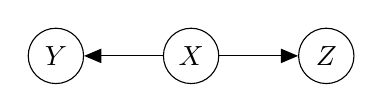
\begin{tikzpicture}
        \node[latent] (X) {$X$};
        \node[latent, left = of X] (Y) {$Y$};
        \node[latent, right = of X] (Z) {$Z$};

        \edge {X}{Y,Z};
    \end{tikzpicture}
\end{center}



L'analyse des relations d'indépendance conditionnelle dans un réseau bayésien repose sur le critère de
d-séparation \cite{10.5555/534975}. Soient $X, Y, Z$ trois ensembles disjoints de nœuds d'un DAG $\mathcal{G}$.
L'ensemble $Z$ est dit d-séparateur de $X$ et $Y$, noté $\langle X \mid Z \mid Y \rangle_d$, si et seulement
si tout chemin non dirigé entre un nœud de $X$ et un nœud de $Y$ est bloqué par $Z$. Un chemin est dit bloqué
s'il existe un nœud $W$ sur ce chemin vérifient l’une des deux conditions suivantes : $W$ est un nœud en collision,
c'est-à-dire qu'il existe dans $\mathcal{G}$ deux arêtes entrantes vers $W$ le long du chemin considéré, autrement dit,
une structure de la forme $A \to W \gets B$, et qu'aucun nœud parmi $W$ et ses descendants n'appartient à $Z$,
ou bien, $W$ n'est pas un nœud en collision et $W$ appartient à $Z$.

Cette caractérisation graphique équivaut à l'indépendance conditionnelle dans l'espace probabiliste

$$
    X \perp Y \iff Z \text{ d-sépare } X \text{ et } Y
$$

\subsection{Apprentissage des BN}

L'apprentissage d'un réseau bayésien à partir de données est un problème NP-complet. Cela a été prouvé par \citet{chickering1996learning}. Cette complexité provient de l'explosion du nombre de structures possibles,
qui croît exponentiellement avec le nombre de variables.Malgré cette complexité inhérente, plusieurs approches heuristiques ont
été développées pour approximer la solution optimale.

\subsubsection{Classes d'Équivalence de Markov}

Dans un réseau bayésien, la structure d'un DAG encode un ensemble d'indépendances conditionnelles à travers le critère de
d-séparation. Toutefois, une même distribution de probabilités peut être représentée par plusieurs DAGs distincts qui
induisent exactement les mêmes relations d'indépendance conditionnelle. Cette propriété conduit à la notion de classe
d'équivalence de Markov.

Deux DAGs $\mathcal{G}_1$ et $\mathcal{G}_2$ sont dits Markov-équivalents si et seulement si ils induisent le même ensemble
d'indépendances conditionnelles. Autrement dit, ils définissent la même factorisation de la loi de probabilité jointe et
conduisent aux mêmes relations d'indépendance entre variables.

Un élément clé pour l'analyse des classes d'équivalence est la notion de v-structure. Soient $A, B$ et $C$ trois variables
dans un DAG $\mathcal{G}$, telles que $A$ et $B$ sont adjacents, $B$ et $C$ sont adjacents, mais aucune arête ne relie
directement $A$ et $C$. Dans ce cas, quatre configurations sont possibles pour l'orientation des arêtes entre ces trois
variables, illustrées dans la Figure \ref{fig:v_structure}. D'un point de vue probabiliste, les trois premières configurations sont indistinguables
en ce qu'elles encodent exactement la même relation d'indépendance conditionnelle, à savoir

$$
    A \perp C \mid B.
$$

En revanche, la quatrième configuration se distingue des autres, car elle encode une relation d'indépendance différente,
en particulier

$$
    A \not\perp C \mid B.
$$

Dans cette dernière structure, le nœud $B$ est un nœud en collision, c'est-à-dire qu'il possède deux arêtes entrantes, et
il n'existe aucune arête directe entre $A$ et $C$. Une telle configuration est appelée une v-structure.

Le théorème de caractérisation de \citet{10.5555/534975} établit un critère nécessaire et suffisant pour que deux DAGs soient
Markov-équivalents. Deux DAGs $\mathcal{G}_1$ et $\mathcal{G}_2$ sont Markov-équivalents si et seulement si ils vérifient
simultanément les deux conditions suivantes :

\begin{enumerate}[label=(\roman*)]
    \item $\mathcal{G}_1$ et $\mathcal{G}_2$ possèdent le même squelette, c'est-à-dire qu'ils admettent le même graphe non orienté
          sous-jacent, où seules les connexions entre variables sont considérées, indépendamment de l'orientation des arêtes.
    \item $\mathcal{G}_1$ et $\mathcal{G}_2$ contiennent exactement les mêmes v-structures
\end{enumerate}


Ces deux conditions garantissent que les DAGs appartenant à une même classe d'équivalence sont indistinguables d'un point de
vue probabiliste, dans la mesure où ils induisent les mêmes relations d'indépendance conditionnelle.


\begin{figure}
    \centering
    \begin{subfigure}[b]{0.45\textwidth}
        \centering
        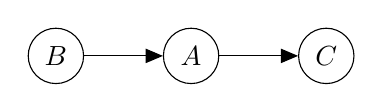
\begin{tikzpicture}[every node/.style={latent}]
            \node (B) {$A$};
            \node (A) [left=of B] {$B$};
            \node (C) [right=of B] {$C$};
            \edge {A}{B};
            \edge {B}{C};
        \end{tikzpicture}
        \caption{}
    \end{subfigure}
    \hfill
    \begin{subfigure}[b]{0.45\textwidth}
        \centering
        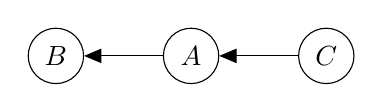
\begin{tikzpicture}[every node/.style={latent}]
            \node (B) {$A$};
            \node (A) [left=of B] {$B$};
            \node (C) [right=of B] {$C$};
            \edge {B}{A};
            \edge {C}{B};
        \end{tikzpicture}
        \caption{}
    \end{subfigure}
    \hfill
    \begin{subfigure}[b]{0.45\textwidth}
        \centering
        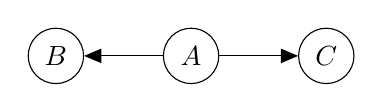
\begin{tikzpicture}[every node/.style={latent}]
            \node (B) {$A$};
            \node (A) [left=of B] {$B$};
            \node (C) [right=of B] {$C$};
            \edge {B}{A,C};
        \end{tikzpicture}
        \caption{}
    \end{subfigure}
    \hfill
    \begin{subfigure}[b]{0.45\textwidth}
        \centering
        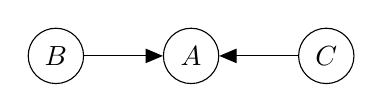
\begin{tikzpicture}[every node/.style={latent}]
            \node (B) {$A$};
            \node (A) [left=of B] {$B$};
            \node (C) [right=of B] {$C$};
            \edge {A}{B};
            \edge {C}{B};
        \end{tikzpicture}
        \caption{}
    \end{subfigure}
    \caption{Configurations d'orientation des arêtes entre $A$, $B$ et $C$. (a)-(c) sont équivalentes; (d) est une v-structure.}
    \label{fig:v_structure}
\end{figure}

\subsection{Approches Basées sur les Contraintes}

Les méthodes d'apprentissage structurel basées sur les contraintes (\textit{constraint-based structure learning}) s'appuient sur
l'identification des indépendances conditionnelles entre variables afin de reconstruire la structure d'un réseau bayésien.
Ces méthodes exploitent le fait que la structure d'un DAG Markov-compatible avec une distribution de probabilités est
entièrement caractérisée par les relations d'indépendance conditionnelle entre variables.

L'algorithme suit généralement trois phases successives :

\begin{enumerate}
    \item Construction du squelette \\
          On détermine d'abord le squelette du graphe, c'est-à-dire son graphe sous-jacent non orienté,
          en effectuant des tests d'indépendance conditionnelle sur les données. Deux variables sont
          reliées par une arête dans le squelette si et seulement si elles ne sont pas indépendantes
          conditionnellement à un sous-ensemble approprié des autres variables observées. Cette phase
          fournit une première approximation de la structure du réseau sans information directionnelle.

    \item Orientation des v-structures\\
          Une fois le squelette obtenu, il est nécessaire d'identifier et d'orienter les v-structures,
          qui sont les seules configurations dont l'orientation est déductible directement à partir des
          relations d'indépendance conditionnelle observées. Ces orientations sont imposées de manière
          unique afin de préserver les relations d'indépendance et de dépendance induites par les tests effectués.

    \item Orientation des arêtes restantes
          Après l'identification des v-structures, les autres arêtes du graphe doivent être orientées en respectant
          deux contraintes fondamentales :
          \begin{enumerate}[label=(\roman*)]
              \item préserver l'acyclicité, c'est-à-dire éviter la formation de cycles dirigés, et
              \item ne pas introduire de nouvelles v-structures non justifiées par les indépendances conditionnelles observées.
          \end{enumerate}

          Pour cela, des règles d'orientation supplémentaires sont appliquées de manière itérative, comme la propagation des
          orientations dérivées des relations d'indépendance.
\end{enumerate}



L'exactitude de ces méthodes dépend fortement de la fiabilité des tests d'indépendance, qui peuvent être affectés par le
bruit ou la taille limitée des échantillons. Dans certains cas, elles ne permettent pas d'orienter toutes les arêtes,
ce qui conduit à l'obtention d'un DAG partiellement orienté (\textit{partially directed acyclic graph}, PDAG), représentant
l'ensemble des structures Markov-équivalentes compatibles avec les données.

\subsubsection{Approches Basées sur les Scores}

Les méthodes basées sur les scores (\textit{score-based}) nous font voir l'apprentissage d'une structure comme un problème
d'optimisation. L'objectif est alors de trouver la structure qui maximise un score reflétant l'adéquation du modèle aux données.

Les scores couramment utilisés sont :

Le score BIC (\textit{Bayesian Information Criterion})\\
Le score BDe (\textit{Bayesian Dirichlet equivalent})\\
Le score MDL (\textit{Minimum Description Length})

Concrètement, ces scores équilibrent deux objectifs contradictoires: trouver un modèle qui s'ajuste bien aux données observées
et éviter les structures trop complexes qui "mémoriseraient" les données plutôt que d'en capturer les tendances générales.

Parmi les algorithmes d'apprentissage basés sur les scores, le GES (\textit{Greedy Equivalence Search}) se démarque par son
efficacité. Au lieu de chercher dans l'immense espace de tous les graphes dirigés possibles, GES procède de façon plus
intelligente en explorant l'espace des classes d'équivalence. L'idée fondamentale est simple : plutôt que de considérer
séparément des graphes qui représentent exactement les mêmes relations de dépendance, GES les traite
comme une seule entité. Cette approche réduit le nombre de structures à évaluer, ce qui permet d'obtenir un bon résultat
même avec un grand nombre de variables.

\bibliographystyle{agsm}
\bibliography{references.bib}


\end{document}